%%%%%%%%%%%%%%%%%%%%%%%%%%%%%%%%%%%%%%%%%%%%%%%%%%%%%%%%%%%%%%%%
% Tipo de documento y paquetes
\documentclass[10pt]{book}
\usepackage{cdt/cdtAnalisis}
\usepackage{subfigure}
\usepackage{appendix}

%%%%%%%%%%%%%%%%%%%%%%%%%%%%%%%%%%%%%%%%%%%%%%%%%%%%%%%%%%%%%%%%
% Datos del proyecto
\sistema[Etapa 1]{Investigación y Desarrollo de un Modelo Ubicuo de Interoperabilidad para la Gestión de un Sistema de Información Institucional}

\documento{DA}{Documento de Análisis--Prototipo de una aplicación móvil de arquitectura offline para desastres naturales}{\DRAFT{\today}} %\RELEASE{1.0}


\fecha{\today}
\proyecto[Trabajo Terminal 2017-B017]{Trabajo Terminal 2017-B017}

\organizacion{Instituto Politécnico Nacional}

\author{Escuela Superior de Cómputo}

	\elaboro[Alumno de la ESCOM]{Eduardo Pérez Gómez}   % Responsable del contenido (IPN)
	\elaboroo[Alumno de la ESCOM]{Héctor Iván Jiménez Romero}
\superviso[Director]{M. en C. Ulises Vélez Saldaña} % Quien recibe el documento (Contraparte)
\sinI[Sinodal]{M. en C. Hermes Fransisco Montes Casiano}
\sinII[Sinodal]{M. en C. Jaime Hugo Puebla Lomas}
\sinIII[Sinodal]{M. en C. Alejandro Sigfrido Cifuentes}
\aprobo[Comité]{ } % Responsable Técnico (Contraparte)

\title{\varProyecto}
\subtitle {\varCveDocumento--\varDocumento}

%\setImgPortada{calmecacTheme/banner2}
%\setImgPleca{calmecacTheme/footer3}
%\setImgHeader{calmecacTheme/logoPar}{calmecacTheme/logoInp}
%\setImgLogo{calmecacTheme/headerInp}{calmecacTheme/headerPar}

%%%%%%%%%%%%%%%%%%%%%%%%%%%%%%%%%%%%%%%%%%%%%%%%%%%%%%%%%%%%%%%
% Elementos contenidos en el documento

%%%%%%%%%%%%%%%%%%%%%%%%%%%%%%%%%%%%%%%%%%%%%%%%%%%%%%%%%%%%%%%%
% Documentos relacionados con el documento actual

%%%%%%%%%%%%%%%%%%%%%%%%%%%%%%%%%%%%%%%%%%%%%%%%%%%%%%%%%%%%%%%%
% Inicio del Documento
\begin{document}

    %=========================================================
    % Portada
    \thispagestyle{empty}

    \maketitle
    
    %=========================================================
    % Hoja de revisión
    \makeDocInfo
    \bigskip\\
    %\makeElemRefs
    %\makeDocRefs
    \makeObservaciones[3cm]
    \vspace{2cm}
    \makeFirmas

    %=========================================================
    % Indices del documento
    \frontmatter
    \tableofcontents
    \listoffigures
    %\listoftables
    \mainmatter

    %=========================================================
    % Para ocultar la información del documentador se descomenta: \hideControlVersion
    %\hideControlVersion

    %=========================================================
    % CAPÍTULOS DEL DOCUMENTO
    \chapter{Planteamiento del problema}
    \label{ch:planteamiento}
	% introduccion.tex
%
% Describe el objetivo, alcance y contenido del documento.
%
%---------------------------------------------------------

%=========================================================
%---------------------------------------------------------
\chapter{Diagramas BPMN}
\label{chapter:bpmn}

	Los diagramas BPMN\footnote{Notación para el Modelado de Procesos de Negocio o BPMN por sus siglas en Inglés (Business Process Modeling Notation).} son una notación gráfica estandarizada que permite el modelado de procesos de negocio en un formato de flujo de trabajo. El objetivo es proporcionar una notación estándar que sea fácilmente legible y entendible por parte de todos los involucrados e interesados del negocio.\\

	Los diagramas BPMN, a diferencia de los diagramas de flujo, permiten modelar el flujo de información entre diversas áreas y organizaciones, el tiempo que toma realizar cierta tarea y los productos generados. Por lo que se determinó la conveniencia de modelar el proceso del CALMÉCAC a través de este estándar.

%\noindent Los diagramas BPMN tienen la característica de mostrar la interacción existente entre las diferentes áreas, entidades o actores de la organización, esto permite visualizar el flujo de la información a través de las áreas.\\

%---------------------------------------------------------
\section{Procesos, Subprocesos y Tareas}

{\bf Proceso.} Es una serie de actividades (coordinadas u organizadas) bien definidas, que se realizan (alternativa o simultáneamente) bajo ciertas circunstancias con un fin determinado. Un proceso puede involucrar: ninguno o más de un {\bf subproceso} y una o varias {\bf tareas}.\\
% 	\begin{figure}[!h]
% 	\centering\noindent{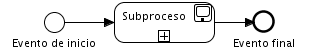
\includegraphics[width=225pt]{introduccion/imagenes/procesos/bpmn/CollapsedSubprocess.png}}%
% 	\caption{Diagrama de un proceso.}
% 	\label{Intro:CollapsedSubprocess}
% 	\end{figure}

{\bf Subproceso.} Es muy similar al {\bf proceso}, con la única diferencia de que éste sólo puede existir o suceder dentro de un proceso. Está representado por la Figura \ref{Intro:iProceso}.\\
 	\begin{figure}[!h]
 	\centering\noindent{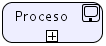
\includegraphics[width=71pt]{introduccion/imagenes/procesos/SubProceso}}%
 	\caption{Representación de un Proceso y/o Subproceso.}
 	\label{Intro:iProceso}
 	\end{figure}
% 	\begin{figure}[!h]
% 	\centering\noindent{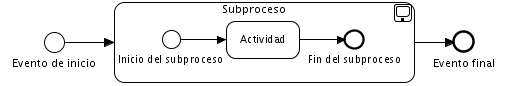
\includegraphics[width=360pt]{introduccion/imagenes/procesos/bpmn/ExpandedSubprocess.png}}%
% 	\caption{Diagrama de un subproceso expandido.}
% 	\label{Intro:ExpandedSubprocess}
% 	\end{figure}

{\bf Tarea o Actividad.} Es el grado de especificación más simple de un proceso (i.e; es el máximo detalle al que puede llegar un proceso) y de ella no pueden derivar más subprocesos o tareas. Está representado por la Figura \ref{Intro:iTarea}.
 	\begin{figure}[!h]
 	\centering\noindent{
\includegraphics[width=68pt]{introduccion/imagenes/procesos/Tarea}}%
 	\caption{Representación de una Tarea.}
 	\label{Intro:iTarea}
 	\end{figure}
% 	\begin{figure}[!h]
% 	\centering\noindent{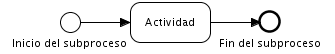
\includegraphics[width=240pt]{introduccion/imagenes/procesos/bpmn/SubprocessDiagram.png}}%
% 	\caption{Diagrama de un subproceso colapsado.}
% 	\label{Intro:CollapsedSubprocess}
% 	\end{figure}


%---------------------------------------------------------
\section{Subprocesos expandidos y contraídos}

{\bf Subproceso expandido.} Los subprocesos en BPMN, pueden representarse como se muestra en la Figura \ref{Intro:ExpandedSubprocess}. Esto significa que un subproceso puede contener varias actividades o subprocesos ``hijos''.
	\begin{figure}[!h]
	\centering\noindent{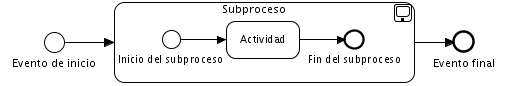
\includegraphics[width=360pt]{introduccion/imagenes/procesos/bpmn/ExpandedSubprocess.png}}%
	\caption{Subproceso expandido.}
	\label{Intro:ExpandedSubprocess}
	\end{figure}

{\bf Subproceso contraído.} Los subprocesos en BPMN, también pueden representarse como se muestra en la Figura \ref{Intro:CollapsedSubprocess}. Esta representación significa lo mismo que la Figura \ref{Intro:ExpandedSubprocess}, pero sin mostrar explícitamente sus actividades o subprocesos ``hijos''.
	\begin{figure}[!h]
	\centering\noindent{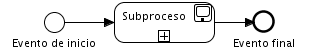
\includegraphics[width=260pt]{introduccion/imagenes/procesos/bpmn/CollapsedSubprocess.png}}%
	\caption{Subproceso contraído.}
	\label{Intro:CollapsedSubprocess}
	\end{figure}

% {\bf Diagrama de un subproceso.} Los subprocesos en BPMN, también pueden representarse como en la Figura \ref{Intro:ExpandedCollapsed}. Esta representación significa lo mismo que la Figura \ref{Intro:ExpandedSubprocess}, pero sin mostrar explícitamente sus actividades o subprocesos ``hijos''.
% 	\begin{figure}[!h]
% 	\centering\noindent{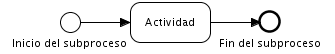
\includegraphics[width=360pt]{introduccion/imagenes/procesos/bpmn/SubprocessDiagram.png}}%
% 	\caption{Intro:Activity}
% 	\label{Intro:CollapsedSubprocess}
% 	\end{figure}


%---------------------------------------------------------
\section{Eventos}

Un {\bf evento} en BPMN representa algo que sucede o podría suceder durante el curso de un proceso y que afecta su flujo. Existen diferentes tipos de eventos:

\begin{itemize}
	\item {\bf Eventos iniciales}. Estos eventos inician el flujo del proceso y no tienen flujos de entrada.

	\arrayrulecolor{white}%
	\begin{tabular}{| m{.08\textwidth} m{.77\textwidth} | }% %{| c{.08\textwidth}  c{.77\textwidth} | }%
		\rowcolor[gray]{0.97}%
		\centering\noindent
\includegraphics[width=18pt]{introduccion/imagenes/procesos/bpmn/StartEvent.png} & {\bf Evento inicial simple}. No se especifica algún comportamiento en particular para empezar un proceso. \\
		\centering\noindent
\includegraphics[width=18pt]{introduccion/imagenes/procesos/bpmn/MessageEventStart.png} & {\bf Evento inicial de mensaje}. Un proceso empieza cuando un mensaje es recibido. \\
		\rowcolor[gray]{0.97}%
		\centering\noindent
\includegraphics[width=18pt]{introduccion/imagenes/procesos/bpmn/TimerEventStart.png} & {\bf Evento inicial de tiempo}. Un proceso empieza en determinada fecha o tiempo específico. \\
		\centering\noindent
\includegraphics[width=18pt]{introduccion/imagenes/procesos/bpmn/RuleEventStart.png} & {\bf Evento intermedio de regla de negocio}. Un proceso inicia cuando una condición de negocio se cumple. \\
		\rowcolor[gray]{0.97}%
		%LINK
		\centering\noindent
\includegraphics[width=18pt]{introduccion/imagenes/procesos/bpmn/LinkEventStart.png} & {\bf Evento inicial de link}. \\
		\centering\noindent
\includegraphics[width=18pt]{introduccion/imagenes/procesos/bpmn/MultipleEndEvent.png} & {\bf Evento inicial múltiple}. Indica que existen muchas formas de iniciar el proceso y que al cumplirse una de ellas se iniciará el proceso. \\
	\end{tabular}%

	\item {\bf Eventos intermedios}. Indican que algo ocurre o podría ocurrir en alguna parte del proceso (desde el inicio y hasta el final). Estos eventos pueden ser usados como parte del flujo de secuencia o adjuntarse a los bordes de una actividad para indicar que la actividad se ejecuta una vez que el evento es activado.

	\arrayrulecolor{white}%
	\begin{tabular}{| m{.08\textwidth} m{.77\textwidth} | }%
		\rowcolor[gray]{0.97}%
		\centering\noindent
\includegraphics[width=18pt]{introduccion/imagenes/procesos/bpmn/IntermediateEvent.png} & {\bf Evento intermedio sin especificar}. Indica algo que ocurre o puede ocurrir dentro del proceso, sólo se pueden utilizar dentro de la secuencia del flujo. \\
		\centering\noindent
\includegraphics[width=18pt]{introduccion/imagenes/procesos/bpmn/MessageEvent.png} & {\bf Evento intermedio de mensaje}. Indica que un mesaje puede ser enviado o recibido en alguna parte del proceso. \\
		\rowcolor[gray]{0.97}%
		\centering\noindent
\includegraphics[width=18pt]{introduccion/imagenes/procesos/bpmn/TimerEventIntermediate.png} & {\bf Evento intermedio de tiempo}. Indica que el proceso debe esperar un tiempo especifico para poder continuar.\\
		\centering\noindent
\includegraphics[width=18pt]{introduccion/imagenes/procesos/bpmn/ErrorIntermediateEvent.png} & {\bf Evento intermedio de error}. Eta figura es usada para capturar errores. Se diagrama a los límites de una actividad. \\
		\rowcolor[gray]{0.97}%
		\centering\noindent
\includegraphics[width=18pt]{introduccion/imagenes/procesos/bpmn/CancelIntermediateEvent.png} & {\bf Evento intermedio de cancelación}. Este tipo de evento intermedio es usado en subprocesos Transaccionales. Se diagrama a los límites del Subproceso transaccional indicando un flujo alternativo que se realizaría cuando el subproceso transaccional es cancelado. Se diagrma a los límites del subproceso. \\
		\centering\noindent
\includegraphics[width=18pt]{introduccion/imagenes/procesos/bpmn/CompensationIntermediateEvent.png} & {\bf Evento intermedio de compensación}. Permite manejar compensaciones. Puede ser usado dentro de la secuencia del flujo para indicar que se requiere una compensación, o adjuntado a los bordes de una actividad para indicar que la actividad será compensada una vez que el evento sea activado.\\
		\rowcolor[gray]{0.97}%
		\centering\noindent
\includegraphics[width=18pt]{introduccion/imagenes/procesos/bpmn/ConditionalIntermediateEvent.png} & {\bf Evento intermedio de condición}. Se usa cuando el flujo necesita esperar por una condición de negocio para ser completado. Sólo puede usarse dentro de la secuencia del flujo o adjuntado a los bordes de una actividad para indicar que existe un flujo de excepción. \\
		\centering\noindent
\includegraphics[width=18pt]{introduccion/imagenes/procesos/bpmn/LinkIntermediateEvent.png} & {\bf Evento intermedio de condición}. Este evento permite conectar dos secciones del proceso y puede ser usado únicamente dentro del flujo del proceso.\\
		\rowcolor[gray]{0.97}%
		\centering\noindent
\includegraphics[width=18pt]{introduccion/imagenes/procesos/bpmn/MultipleIntermediateEvent.png} & {\bf Evento intermedio múltiple}. Este evento puede ser activado por muchas causas o sólo por una de ellas. Sólo puede usarse dentro de la secuencia del flujo.\\
	\end{tabular}%

	\item {\bf Eventos finales}. Estos eventos finalizan el flujo del proceso, por lo tanto no pueden tener flujos de salida.

	\arrayrulecolor{white}%
	\begin{tabular}{| m{.08\textwidth} m{.77\textwidth} | }%
		\rowcolor[gray]{0.97}%
		\centering\noindent
\includegraphics[width=18pt]{introduccion/imagenes/procesos/bpmn/End.png} & {\bf Evento final sin especificar.} Indica que un camino del flujo llego al fin. \\
		\centering\noindent
\includegraphics[width=18pt]{introduccion/imagenes/procesos/bpmn/MessageEndEvent.png} & {\bf Evento de in de mensaje.} Permite enviar un mensaje al finalizar el flujo.\\
		\rowcolor[gray]{0.97}%
		\centering\noindent
\includegraphics[width=18pt]{introduccion/imagenes/procesos/bpmn/ErrorEndEvent.png} & {\bf Evento de fin de error.} Permite enviar una excepción de error al finalizar el flujo. \\
		\centering\noindent
\includegraphics[width=18pt]{introduccion/imagenes/procesos/bpmn/CancelEndEvent.png} & {\bf Evento final de cancelación}. Permite enviar una excepción de error cuando el flujo llega al final. Este evento solo puede usarse en subprocesos. \\
		\rowcolor[gray]{0.97}%
		\centering\noindent
\includegraphics[width=18pt]{introduccion/imagenes/procesos/bpmn/CompensationEndEvent.png} & {\bf Evento de fin de compensación.} Este tipo de fin indica que es necesaria una compensación al finalizar el flujo. \\
		\centering\noindent
\includegraphics[width=18pt]{introduccion/imagenes/procesos/bpmn/LinkEvent.png} & {\bf Evento final de liga}. Este evento permite conectar dos secciones del proceso. Sólo puede usarse dentro del flujo del proceso.\\
		\rowcolor[gray]{0.97}%
		\centering\noindent
\includegraphics[width=18pt]{introduccion/imagenes/procesos/bpmn/EndEvent.png} & {\bf Evento final.} Indica que el proceso y todas las actividades terminan, sin importar que alguna haya quedado pendiente. \\
		\centering\noindent
\includegraphics[width=18pt]{introduccion/imagenes/procesos/bpmn/MultipleEndEvent.png} & {\bf Evento de fin múltiple} Indica que varios resultados pueden darse al finalizar un flujo. \\

	\end{tabular}%
\end{itemize}

%---------------------------------------------------------
\section{Compuertas}

Las {\bf compuertas} son elementos usados para controlar la divergencia y convergencia del flujo (separar y unir).\\

	\arrayrulecolor{white}%
	\begin{tabular}{| m{.08\textwidth} m{.77\textwidth} | }%
		\rowcolor[gray]{0.97}%
		\centering\noindent
\includegraphics[width=25pt]{introduccion/imagenes/procesos/bpmn/ExclusiveGateway.png} & {\bf Compuerta exclusiva basado en los datos}. Como decisión exclusiva, tiene dos o más flujos de secuencia alternos, pero solo uno de ellos puede tomarse basado en la condición de los datos. Como convergencia, es usado para mezclar rutas alternas en una sola. \\
		\centering\noindent
\includegraphics[width=25pt]{introduccion/imagenes/procesos/bpmn/EventBasedGateway.png} & {\bf Compuerta exclusiva basada en eventos}. Representa un punto del proceso donde se escoge un camino de varios disponibles, pero la decisión no se basa en datos del proceso sino en eventos.\\
		\rowcolor[gray]{0.97}%
		\centering\noindent
\includegraphics[width=25pt]{introduccion/imagenes/procesos/bpmn/InclusiveGateway.png} & {\bf Compuerta inclusiva}. Como divergencia, es usada cuando en un punto del flujo una o más rutas puden ser activadas y la decisión está basada en los datos del proceso. Como convergencia, indica que las rutas activas son sincronizadas en una sola.\\
		\centering\noindent
\includegraphics[width=25pt]{introduccion/imagenes/procesos/bpmn/ComplexGateway.png} & {\bf Compuerta compleja}. Como divergencia, es utilizada para controlar puntos de decisión complejo. Como convergencia, permite continuar al siguiente punto del proceso cuando una condición de negocio se cumple.\\
		\rowcolor[gray]{0.97}%
		\centering\noindent
\includegraphics[width=25pt]{introduccion/imagenes/procesos/bpmn/ParallelGateway.png} & {\bf Compuerta paralela}. Como divergencia, es usada para crear rutas paralelas. Como convergencia, sincroniza multiples rutas paralelas en una. El flujo continúa cuando todas las rutas alcanzan la compuerta. \\
	\end{tabular}%

%---------------------------------------------------------
\section{Conectores}

Los {\bf conectores} son elementos usados para conectar objetos (tareas, subprocesos, eventos, compuertas, etc.) dentro del flujo.\\

	\arrayrulecolor{white}%
	\begin{tabular}{| m{.33\textwidth}  m{.52\textwidth} | }%
		\rowcolor[gray]{0.97}%
		\centering\noindent
\includegraphics[width=120pt]{introduccion/imagenes/procesos/bpmn/SequenceFlow.png} & {\bf Flujo de secuencia}. Representa el control del flujo y la secuencia de las actividades, compuertas y eventos. \\
		\centering\noindent
\includegraphics[width=120pt]{introduccion/imagenes/procesos/bpmn/MessageFlow.png} & {\bf Flujo de mensaje}. Es usado para mostrar el flujo de mensajes entre dos entidades o procesos. Representa señales o mensajes, {\bf no el control del flujo}. {\bf No todos los flujos de mensaje son secuenciales o esto especificaría orden en los mensajes}.
	\end{tabular}%


%---------------------------------------------------------
\section{Contenedores}

Un {\bf contenedor} es un elemento utilizado en BPMN para distinguir visualmente las responsabilidades entre las áreas u organizaciones.\\

	\arrayrulecolor{white}%
	\begin{tabular}{| m{.33\textwidth}  m{.52\textwidth} | }%
		\rowcolor[gray]{0.97}%
		\centering\noindent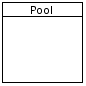
\includegraphics[width=45pt]{introduccion/imagenes/procesos/bpmn/Pool.png} & {\bf Pool}. Un {\it pool} es un contenedor representando un sólo proceso. \\%El nombre del {\it pool} puede ser considerado el nombre del proceso. \\
		\centering\noindent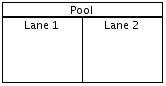
\includegraphics[width=70pt]{introduccion/imagenes/procesos/bpmn/Lane.png} & {\bf Lane}. Un {\it lane} es una subdivisión de un {\it pool} y representa un rol o área organizaquecional.
	\end{tabular}%


%- - - - - - - - - - -  - - - - - - - - - -  - - - - -

\section{Código de Colores}
\label{section:CodigoColores}

\subsection{Arquitecturas}

Para la arquitectura, los \textit{pools} horizontales representan el área o departamento encargado del proceso, los \textit{lanes} representan el proceso que se modelará.\\
El relleno(\textit{fill}) de estos elementos deberá ser \textit{Grandient Light Blue} con el 80\% de transparencia como se muestra en la figura \ref{fig:poolProceso}. Color 1 del gradiente : \textit{RGB(150,223,255)}, color 2  del gradiente: \textit{RGB(102,180,255)}.

\begin{figure}[hbtp!]
	\begin{center}
		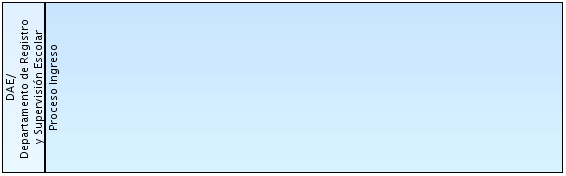
\includegraphics[width=.3\textwidth]{introduccion/imagenes/procesos/PoolProceso}
		\caption{Pool del Proceso}
		\label{fig:poolProceso}
	\end{center}
\end{figure}

Los \textit{pools} verticales representan el área o departamento externo al proceso, el \textit{lane} representa el proceso que realizan estas áreas que aporta al proceso que se desea modelar.\\
El relleno(\textit{fill}) de estos elementos deberá ser \textit{Gradient Gray} con el 80\% de transparencia como se muestra en la figura \ref{fig:poolExterno}. El color 1 del gradiente es \textit{RGB(245,245,245)} y el color 2 \textit{RGB(201,201,201)}.

\begin{figure}[hbtp!]
	\begin{center}
		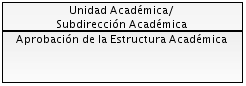
\includegraphics[width=.3\textwidth]{introduccion/imagenes/procesos/PoolExterno}
		\caption{Pool del Proceso Externo}
		\label{fig:poolExterno}
	\end{center}
\end{figure}

El \textit{pool} que se usará para representar al \refElem{Calmecac} utiliza color \textit{RGB(128,0,0)} al 80\% de transparencia como relleno(\textit{fill}) como se muestra en la figura \ref{fig:poolCalmecac}.

\begin{figure}[hbtp!]
	\begin{center}
		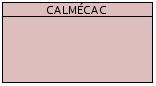
\includegraphics[width=.3\textwidth]{introduccion/imagenes/procesos/PoolCalmecac}
		\caption{Pool del Calmecac}
		\label{fig:poolCalmecac}
	\end{center}
\end{figure}

\section{Macroprocesos y Subprocesos}

Los \textit{pools} representan áreas y departamentos que están involucrados en el proceso y su relleno es \textit{Light Gray} al 80\% de transparencia si son áreas externas y completamente transparentes si son áreas que forman parte del proceso a modelar.
El \refElem{Calmecac} tendrá el mismo color como en la figura \ref{fig:poolCalmecac}.

\section{Cambios}

Para mostrar los cambios en tareas y flechas de comunicación respecto al diagrama anterior se usará una línea de color \textit{RGB(179,89,0)} con un valor de 2 en el peso y las tareas tienen el relleno(\textit{fill})  \textit{Golden} con el 80\% de transparencia como se muestra en la figura \ref{fig:TareasYFlujos}



\begin{figure}[hbtp!]
	\begin{center}
		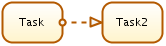
\includegraphics[width=.3\textwidth]{introduccion/imagenes/procesos/ArrowCambios}
		\caption{Flecha para mostrar los cambios}
		\label{fig:TareasYFlujos}
	\end{center}
\end{figure}



 








	
	\chapter{Marco Teórico} 
	\label{ch:marco}
	\section{Sistemas de alarma sísmica}

\section{Transmisión de alarma sísmica}
	
	
	%========Modelo del Negocio ===== %
	\part{Modelo del Negocio}
	
	% Glosario
	\chapter{Glosario}
	\label{chapter:glosario}
	\section{Glosario de términos}

	Esta sección describe de forma breve y sencilla los términos que son usados a lo largo del documento y que se consideran necesario para ayudar a comprender la jerga utilizada en el  CVH.


	
\begin{bGlosario}
	
	\bTerm{Alta}{Alta} Documento que acredita y reconoce la inscripción. %MP DAE
	
	\bTerm{AlumnoRegistradoEnSIRCEI}{Alumno Registrado en SIRCEI} Alumno del nivel medio superior o superior, reconocido en el Sistema de Registro y Control Escolar Institucional, para su control y seguimiento a su trayectoria académica, y consulta de calificaciones, vía internet. %MP DAE
	
	\bTerm{AntecedentesDeIngreso}{Antecedentes de Ingreso} Reseña de la Admisión del alumno en la Institución. % MP DAE
	
	\bTerm{AntecedentesDeTrayectoria}{Antecedentes de Trayectoria} Situación del alumno que ha llevado una dirección dentro del Instituto a lo largo del tiempo. % MP DAE
		
	\bTerm{AspiranteAceptado}{Aspirante Aceptado} Aspirante que al haber aprobado el examen de admisión y que cumple con los requisitos establecidos en la convocatoria correspondiente es asignado a una unidad académica. %Derivado
	
	
	\bTerm{AspiranteAExaminar}{Aspirante a Examinar}Persona que se registra en el proceso de admisión para ingresar a alguna de las escuelas, centros y unidades del Instituto, en los niveles que constituyen su oferta educativa. %MP DAE
	
	\bTerm{Boleta}{Boleta}Cédula de identidad que se otorga a los aspirantes, para que se inscriban como alumnos del Instituto Politécnico Nacional. %MP DAE
	
	\bTerm{Cadena}{Cadena} Es el Tipo de Dato definido por cualquier valor que se componga de una secuencia de caracteres, con o sin acentos, espacios, dígitos y signos de puntuación. Existen tres tipos de Cadenas: Palabra, Frase y Párrafo.
	
	\bTerm{CalendarioAcademico}{Calendario Académico} Programación que define los tiempos en los cuales se realizan anualmente las actividades académicas y de gestión escolar, en las diversas modalidades educativas que se imparten en el Instituto 
	
	\bTerm{CicloEscolar}{Ciclo Escolar} El lapso anual que define el calendario académico
	
	\bTerm{Convocatoria}{Convocatoria} Documento de carácter oficial emitido por una o varias Instituciones Educativas, en el cual se plantea tanto el procedimiento, los tiempos y fechas, los
	lineamientos legales en los que se basa la misma, y los requisitos que hay que cumplir para que un aspirante sea admitido al nivel de estudios superior inmediato concluido por él mismo, en la o las Instituciones que ofrecen sus distintas carreras y niveles de estudios impartidos por las mismas. % MP DAE
	
	\bTerm{CredencialDeAlumno}{Credencial de Alumno} Identificación oficial expedida por la Dirección de Administración Escolar del IPN, para todos aquellos alumnos que cursan alguna carrera en uno de los planteles educativos del Instituto, ya sea a Nivel Medio Superior o Superior. %MP DAE
	
	\bTerm{DictamenDeCategoria}{Dictámen de Categoría} Documento que determina la categoría a la que corresponde un profesor de acuerdo a sus méritos académicos y profesionales. Es expedido por la  Comisión Mixta Paritaria de Evaluación de Categoría Docente. % MANUAL PARA DOCENTES Y COORDINADORES DEL PROCESO DE EVALUACIÓN DE CATEGORÍA DOCENTE
	
	
	\bTerm{Entero}{Entero} Es el Tipo de Dato definido por todos los valores numéricos enteros, tanto positivos como negativos.
	
	\bTerm{EstructuraAcademica}{Estructura Académica} Al conjunto de grupos, horarios y unidades de aprendizaje organizadas para el período siguiente.
	
	\bTerm{ETS}{Examen a Título De Suficiencia} Es la evaluación que comprende el total de los contenidos del programa de estudios y que el alumno podrá presentar cuando no haya acreditado de manera ordinaria o extraordinaria alguna unidad de aprendizaje.
	
	\bTerm{ExpedienteAcademico}{Expediente Académico} Al documento que contiene la información y el historial académico del alumno.
	
	\bTerm{ExpedienteDelAspirante}{Expediente del Aspirante} Se refiere a la documentación que el aspirante entrega durante el proceso de admisión para su verificación. % Derivado
	
	\bTerm{Fecha}{Fecha} Es el Tipo de Dato definido por todas las fecha pasadas y futuras. Se representa de dos formas: Fecha Corta y Fecha Larga.
	
	\bTerm{FechaCorta}{Fecha corta} Representación de una fecha de la forma DD/MM/YYYY, ejemplo: 24/02/2012.
	
	\bTerm{FechaLarga}{Fecha Larga} Representación de una fecha de la forma DD de MMMM, del YYYY, ejemplo: 24 de Febrero, del 2012.
	
	\bTerm{Frase}{Frase} Cadena formada por mas de una palabra y que puede ocupar hasta un par de renglones.
	
	\bTerm{HistorialAcademico}{Historial Académico} Se entiende por historial académico al conjunto de calificaciones obtenidas por un alumno en las unidades de aprendizaje,durante su vida académica dentro del Instituto.
	
	\bTerm{HojaDeResultadoDelExamenDeAdmision}{Hoja de Resultado del Examen de Admisión} Documento que el interesado imprime a través de internet, para conocer la opción educativa donde quedó aceptado. Con la Hoja de Resultados los aspirantes seleccionados obtendrán una cita donde podrán continuar con sus trámites de inscripción al Instituto. %MP DAE
	
	\bTerm{Horario}{Horario} Documento que se le otorga a un aspirante o alumno en el que se confirma su inscripción al período en curso.
	
	\bTerm{Incidencia}{Incidencia}Acontecimiento que sobreviene en el curso de un asunto o negocio y tiene con él alguna conexión.
	
	
	\bTerm{Kardex}{Kardex} Documento donde se resgistran los datos personales del alumno, el cual contiene la trayectoria escolar mediante las calificaciones obtenidas en las asignaturas y/o unidades de aprendizaje cursadas, de acuerdo a un plan de estudios, formas de evaluación y periodos escolares. % CIRCULAR NO5 Criterios de Expedición de Boletas de calificaciones
	
	\bTerm{Modalidad}{Modalidad Educativa} Forma en que se organizan, distribuyen y desarrollan los planes y programas de estudio para su impartición. Existen 3 tipos de modalidades:
	\begin{itemize}
		\item [Escolarizada:] La que se desarrolla en aulas, talleres, laboratorios y otros ambientes de aprendizaje, en horarios y periodos determinados.
		\item [No Escolarizada:] Es la que se desarrolla fuera de aulas,
		talleres, laboratorios y no necesariemente comprende horarios determinados.
		\item [Mixta:] Es la combinación de modalidades educativas de
		acuerdo con el diseño un programa académico en particular.
	\end{itemize}
	
	\bTerm{Nombramiento}{Nombramiento} Proceso por el cual un aspirante a dar cátedra en el instituto es elegido otorgándole las horas que deberá cumplir. % RCITPAIPN
	
	
	\bTerm{OficioDeAlumnoAceptado}{Oficio de Alumno Aceptado} Documento generado por la Dirección de Administración Escolar del IPN, por medio del cual el aspirante es notificado que al concluir los trámites de inscripción adquiere el estatus de alumno del Instituto. % MP DAE
	
	\bTerm{PeriodoEscolar}{Periodo Escolar} Lapso señalado en el calendario académico para cursar unidades de aprendizaje de un programa académico.
	
	\bTerm{PlanDeEstudios}{Plan de Estudios} Estructura curricular que se deriva de un programa académico y que permite cumplir con los propósitos de formación general,
	la adquisición de conocimientos y el desarrollo de capacidades correspondientes a un nivel y modalidad educativa.%Reglamento General de Estudios
	
	
	\bTerm{Preboleta}{Preboleta} Es un numéro de identificación que se le asgina al aspirante como fin de control interno durante el proceso de admisión. %Derivado
	
	\bTerm{ProcesoDeAdmision}{Proceso de Admisión} Conjunto de etapas que deben ser realizadas tanto por la Institución educativa como por el aspirante. Comprende desde la publicación de la convocatoria, el regist ro de aspirantes, la aplicación del examen de admisión, publicación de resultados e inscripciones de aspirantes seleccionados. %MP DAE
	
	\bTerm{ProgramaAcademico}{Programa Académico} Al conjunto organizado de elementos necesarios para generar, adquirir y aplicar el conocimiento en un campo específico;así como para desarrollar
	habilidades, actitudes y valores en el alumno, en
	diferentes áreas del conocimiento. %Reglamento General de Estudios
	
	\bTerm{RCITPAIPN}{Reglamento de  las  Condiciones Interiores de Trabajo del Personal Académico del IPN} Reglamento que fija las condiciones de trabajo del personal académico del
	Instituto Politécnico Nacional, que conjuntamente con sus tres anexos:
	\begin{itemize}
		\item[I.] Prestaciones Sociales y Económicas.
		\item[II.] Seguridad e Higiene.
		\item[III.] Promoción Docente.
	\end{itemize}
	Son de observancia obligatoria para el personal académico, el titular y demás funcionarios del Instituto
	Politécnico Nacional y de sus Organos de Apoyo.
	
	\bTerm{RUAA}{Registro Único de Actividades Académicas } Es  el  documento  que  avala  las  funciones  y  actividades  que  desarrolla  el  docente
	
	\bTerm{TrayectoriaEscolar}{Trayectoria Escolar} Al proceso a través del cual el alumno construye su formación con base en un plan de estudio.
	
	\bTerm{UnidadDeAprendizaje}{Unidad de Aprendizaje} A la estructura didáctica que integra los contenidos formativos de un curso, materia, módulo, asignatura o sus equivalentes.
	En general, las unidades de aprendizaje deberán cursarse y acreditarse conforme lo establezca el plan de estudio, y podráan seleccionarse de entre
	la oferta disponible en el periodo escolar y sujeta a grupo. %Reglamento General de Estudios
	
	\bTerm{ValidacionDeInscripcion}{Validación de Inscripción} Proceso a través del cual se dictamina la autenticidad y legitimidad de los documentos aportados por el aspirante para su inscripción, si la documentación es correcta se le comunica por escrito. %MP DAE
	
	
	
	% TODO:Agregar fuente
	
 
\end{bGlosario}



				%Glosario de términos técnicos y del negocio
	
	
	% Modelo de Información
	
	\chapter{Modelo de Información} %Diagrama de Clases
	\label{chapter:modeloInformacion}
	% Modelo Estructural
	
	
	%Reglas de Negocio
	\chapter{Reglas de Negocio} % Reglas de Negocio
	\label{chapter:rn}
	% No comentar las reglas cuyo estatus es APROBADO.
%Ejemplo de regla de negocio

%Este documento llamará a las reglas

\section{Introducción al Capítulo}

Bla bla bla....


\section{Reglas de la DAE}
	\begin{BusinessRule}{BR100}{Recibo del Estudiante por inscripción a Seminario.}{
		Regla de operación, (calcular o determinar un valor.).
		% Otras opciones para tipo: 
		% - Regla de integridad referencial o estructural. 
		% - Regla de operación, (calcular o determinar un valor.).
		% - Regla de inferencia de un hecho.
	}{
		Habilitadora. 
		% Otras opciones para clase: Habilitadora, Cronometrada, Ejecutive.
	}{
		Controla la operación. % Otras opciones para nivel: Controla la operación, Influencia (dirige) la operación.
	}
	\BRItem[Descripción:] El  Recibo del Estudiante debe mostrar el total del costo con el siguiente desglose:
	\begin{displaymath}\begin{array}{lr}
	Costo: & \$ XXX.XX\\
	Descuento~aplicado~(YY\%): & \$ XXX.XX\\
	Subtotal: & \$ XXX.XX\\
	IVA~(16\%): & \$ XXX.XX\\\hline
	Total: & \$ XXX.XX
	\end{array}\end{displaymath}
	\BRItem[Sentencia:] $CostoTotal = Costo(e, s) + Impuesto(e, s)$.
	\BRItem[Ejemplo positivo:] 
	
	\BRItem[Ejemplo negativo:] 
	
	\BRItem[Referenciado por:] 
\end{BusinessRule}
	
	
\section{Reglas de la DEMS}




	
	%======Modelo Dinámico ===== %
	\part{Modelo Dinámico}
	
	
	%Modelo de Casos de Uso
	\chapter{Modelo de Casos de Uso} % Casos de Uso
	\label{chapter:UC}
	\section{Introducción al Capítulo}
Bla bla bla....
%Diagrama de Casos de Uso


	
	
	%Actores
	\chapter{Modelado de Actores}
	\label{chapter:actores}
	%=============================================
% Descripción de actores
\label{chapter:ActoresDelSistema}

	En el presente capítulo se definen los participantes en los procesos actuales y fortalecidos. Se da una breve descripción de cada uno, la mayoría tomada de la normatividad correspondiente: Reglamento General, Reglamento interno y Manuales de operación del IPN, entre otros. Aquellas descripciones tomadas de la normatividad tienen la referencia del documento de dónde fueron tomadas.

\section{Descripción de participantes}

Cada participante se describe con la siguiente estructura:

\begin{objetivos}[Descripción de participantes]
	\item {\bf Nombre:} Nombre con el que se le conoce al participante dentro del negocio.
	\item {\bf Descripción:} Descripción breve del perfil, puesto o rol que juega el participante.
\end{objetivos}

\section{Participantes detectados}

\begin{actor}{ciudadano}{Ciudadano}{
		Persona que habita en la Ciudad de México.
}	
\end{actor}

	
	
	%Estados
	\chapter{Modelo de Estados} % Estados
	\label{chapter:edos}
	
	%Capitulo por cada CU
	\chapter{Casos de Uso}
	%Entradas
\begin{UseCase}{CU25}{Configurar alertas sísmicas}{
		Permite realizar la configuración de una alerta sísmica que le servirá al actor cuando llegue a haber un sismo en la ciudad y de esta manera pueda saber que habrá un sismo y pueda buscar algún refugio cercano. \\
		
		Al configurar una alerta sísmica el actor podrá elegir el tono en el que esta sonará cada vez que haya un sismo. \\
}
	\UCitem{Versión}{0.1}
	\UCccsection{Datos para el control Interno}	
	\UCitem{Autor}{Alberto García Paul}
	\UCccitem{Evaluador}{Ulises Veléz Saldaña}
	\UCitem{Operación}{Configurar}
	\UCccitem{Prioridad}{Alta}
	\UCccitem{Complejidad}{Media}
	\UCccitem{Volatilidad}{Media}
	\UCccitem{Madurez}{Media}
	\UCitem{Estatus}{Edición}
	\UCitem{Fecha del último estatus}{26 de marzo de 2018}
	\UCccsection{Revisión Version 0.1}
	\UCccitem{Fecha}{}
	\UCccitem{Evaluador}{Ulises Veléz Saldaña}
	\UCccitem{Resultado}{}
	\UCccitem{Observaciones}{}
	\UCsection{Atributos}
	\UCitem{Actor(es)}{\refElem{ciudadano}}
	\UCitem{Propósito}{Contar con un medio en el que el actor pueda configurar la alerta sísmica desea que suene cuando haya un sismo}
	\UCitem{Entradas}{Ninguna}
	\UCitem{Origen}{No aplica}
	\UCitem{Salidas}{Mensaje de confirmación.}
	\UCitem{Precondiciones}{Ninguna}
	\UCitem{Postcondiciones}{Se configurará la nueva alerta sísmica}
	\UCitem{Reglas de Negocio}{Ninguna}
	\UCitem{Errores}{Ninguno}
	\UCitem{Disparador(es)}{}
	\UCitem{Condiciones de Término}{Se muestra el mensaje 1 en pantalla}
	\UCitem{Efectos Colaterales}{Se podrá configurar el tono de la alerta sísmica.}
	
\end{UseCase}


%Trayectoria Principal : Happy Path

\begin{UCtrayectoria}
	\UCpaso Revisa la lista de usuarios que desean recibir notificaciones.\refTray{A}
	\UCpaso Notifica al \UCactor que debe realizar la inscripción de aspirantes con el mensaje Cargar Aspirantes.
	\item \UCactor Ingresa al Calmécac.\refTray{B}
	\UCpaso Le
\end{UCtrayectoria}


\begin{UCtrayectoriaA}{A}{Cuando no existen mensajes}
	\UCpaso lalala
	\item \UCactor lololol
\end{UCtrayectoriaA}

%

\begin{UseCase}{CU10}{Inscribir Aspirante}{
		Este caso de uso ayudará al \refElem{DepartamentoDeGestionEscolar} a ingresar el registro de los aspirantes admitidos a los horarios creados por el proceso de estructura académica \refElem{Calmecac}.
}
	\UCitem{Versión}{0.1}
	\UCccsection{Datos para el control Interno}	
	\UCitem{Autor}{Francisco Isidoro Mera Torres}
	\UCccitem{Evaluador}{Ulises Veléz Saldaña}
	\UCitem{Operación}{Gestionar}
	\UCccitem{Prioridad}{Alta}
	\UCccitem{Complejidad}{Media}
	\UCccitem{Volatilidad}{Media}
	\UCccitem{Madurez}{Media}
	\UCitem{Estatus}{Edición}
	\UCitem{Fecha del último estatus}{28 de Junio del 2017}
	\UCccsection{Revisión Version 0.1}
	\UCccitem{Fecha}{}
	\UCccitem{Evaluador}{Ulises Veléz Saldaña}
	\UCccitem{Resultado}{}
	\UCccitem{Observaciones}{}
	\UCsection{Atributos}
	\UCitem{Actor(es)}{\refElem{DepartamentoDeGestionEscolar},\refElem{Aspirante}}
	\UCitem{Propósito}{Proporcionar al \refElem{DepartamentoDeGestionEscolar} un mecanismo para a inscribir a los aspirantes de acuerdo a un criterio si existe o realizar esta tarea manualmente}
	\UCitem{Entradas}{Estructura Académica, Aspirantes con preboleta}
	\UCitem{Salidas}{Aspirante con Horario}
	\UCitem{Precondiciones}{
		\begin{Titemize}
			\Titem La estructura académica debe estar cargada en el \refElem{Calmecac}
			\Titem Los aspirantes deben tener un número de \refElem{Preboleta}\footnote{Esto implica que debieron haber sido aceptados}
		\end{Titemize}}
	\UCitem{Postcondiciones}{El aspirante queda inscrito con un \refElem{Horario}}
	\UCitem{Reglas de Negocio}{}
	\UCitem{Errores}{
		\begin{Titemize}
			\Titem \UCerr{Uno}{Cuando no existe o no ha sido carga la estructura académica en el sistema}{el Calmécac enviará el mensaje \textbf{Elementos no Disponibles}}
			\Titem \UCerr{Dos}{Cuando no existen aspirantes cargados en el sistema}{el Calmécac enviará el mensaje \textbf{Elemetos no Disponibles}}
		\end{Titemize}
		}
	\UCitem{Tipo}{}
	\UCitem{Disparador(es)}{}
	\UCitem{Issues}{}
	\UCitem{Requerimientos no Funcionales}{}
	\UCitem{Requerimientos de Usuario}{}
	\UCitem{Condiciones de Término}{}
	\UCitem{Efectos Colaterales}{}
	
\end{UseCase}


%Trayectoria Principal : Happy Path

\begin{UCtrayectoria}
	\UCpaso Revisa la lista de usuarios que desean recibir notificaciones.\refTray{A}
	\UCpaso Notifica al \UCactor que debe realizar la inscripción de aspirantes con el mensaje Cargar Aspirantes.
	\item \UCactor Ingresa al Calmécac.\refTray{B}
	\UCpaso Le
\end{UCtrayectoria}


\begin{UCtrayectoriaA}{A}{Cuando no existen mensajes}
	\UCpaso lalala
	\item \UCactor lololol
\end{UCtrayectoriaA}

	
	%====Modelo de Interacción====%
	\part{Modelo de la Interacción}
	
	
	
	%Entorno de Trabajo
	\chapter{Entorno de Trabajo}
	\label{chapter:entornoTrabajo}
	
	
	%Navegación
	\chapter{Navegación}
	\label{chapter:navegacion}
	
	
	%Diseño de Interfaces
	\chapter{Diseño de Interfaces}
	\label{chapter:interfaces}
	
	%Falta definir entorno mensajes
	\chapter{Diseño de Mensajes}
	\label{chapter:msgs}
	%\chapter{Mensajes del sistema}
\label{chapter:mensajes}
\cdtLabel{apendice:Mensajes}{}


%===========================  MSG1 ==================================
\begin{mensaje}{MSG1}{Elementos No Disponibles}{Error \msgError}
	\item[Canal:] Sistema
    \item[Propósito:] Alertar al actor que no existen elementos en el sistema por mostrar.
    \item[Redacción:] ¡No hay $<ELEMENTOS>$ para mostrarte!
    \item[Parámetros:] ELEMENTOS: Información de la cual se requiere para concluir un proceso
    \item[Ejemplo:] ¡No hay registros de aspirantes para mostrarte!
\end{mensaje}

%============================== MSG2 =================================
\begin{mensaje}{MSG2}{Elemento No Disponible}{Error \msgError}
	\item[Canal:] Sistema
    \item[Propósito:] Alertar al actor que el elemento que se desea ver no existe o no está disponible en el sistema
    \item[Redacción:] ¡Este/a $<ELEMENTO>$ no esta disponible aún!
    \item[Parámetros:] ELEMENTO:Información de un registro en específico de la cual se requiere para concluir un proceso
    \item[Ejemplo:] ¡Esta boleta no esta disponible aún!
\end{mensaje}

%===========================  MSG3 ==================================
\begin{mensaje}{MSG3}{Operación Exitosa}{Confirmación \msgConfirm}
	\item[Canal:] Sistema
    \item[Propósito:] Informar al actor que la operación que se le ha solicitado al sistema se llevo a cabo exitosamente.
    \item[Redacción:] La $<OPERACION>$ se llevo a cabo correctamente.
    \item[Parámetros:] OPERACION: Actividad que el actor debe realizar.
    \item[Ejemplo:] La reincripción se llevo a cabo correctamente.
\end{mensaje}

%============================== MSG4 =================================
\begin{mensaje}{MSG4}{Operación Fallida}{Error \msgError}
	\item[Canal:] Sistema
    \item[Propósito:] Informar al actor que la operación solicitada al sistema no pudo llevarse a cabo.
    \item[Redacción:] Error, $<ERROR\_ENCONTRADO>$.
    \item[Parámetros:] ERROR\_ENCONTRADO: Error que el sistema identificó al intentar realizar la operación.
    \item[Ejemplo:] Error, No hay conexión al sistema.(Base de Datos)
\end{mensaje}

%============================== MSG5 =================================
\begin{mensaje}{MSG5}{Duplicado de Información}{Error \msgError}
	\item[Canal:] Sistema
    \item[Propósito:] Indicar al actor que ya existe un elemento con la misma información que desea ingresar.
    \item[Redacción:] ¡Ya existe un/a $<ELEMENTO>$ con la misma información!
    \item[Parámetros:] ELEMENTO: Parte de la información que esta duplicada
    \item[Ejemplo:]¡Ya existe una boleta con la misma información!
\end{mensaje}

%============================== MSG6 =================================
\begin{mensaje}{MSG6}{Información Incorrecta}{Error  \msgError}
	\item[Canal:] Sistema
	\item[Propósito:] Informar al actor que faltan datos o que los datos proporcionados son érroneos dentro de un formulario.
	\item[Redacción 1:] Falta un dato en el formulario.
	\item[Redacción 2:] La información proporcionada es incorrecta.
	\item[Parámetros:] Ninguno
	\item[Ejemplo:] --
\end{mensaje}

%============================== MSG7 =================================
\begin{mensaje}{MSG7}{Operación por Atender}{Notificación \msgNotif}
	\item[Canal:] Correo / SMS / WhatsApp
	\item[Propósito:] Informar al actor que existen operaciones que requieren de su atención o supervisión para llevarse a cabo.
	\item[Redacción:] Calmécac te notifica que hay $<ELEMENTOS>$ que requieren de tu atención.
	\item[Parámetros:] ELEMENTOS: Aquella información que el actor debe supervisar o atender.
	\item[Ejemplo:] Calmécac te notifica que hay registros de aspirantes que requieren de tu atención.
\end{mensaje}



%===============================MSG8=============================

\begin{mensaje}{MSG8}{Límite de Tiempo}{Notificación \msgNotif}
	\item[Canal:] Correo / SMS / WhatsApp
	\item[Propósito:] Informar al actor que el límite de tiempo para que realize una operación está por agotarse.
	\item[Redacción:]¡ALERTA! Recuerda que debes realizar la $<OPERACION>$ antes del $<TIEMPO>$
	\item[Parámetros:]\cdtEmpty
		\begin{itemize}
			\item OPERACION: Tarea a realizar por el actor
			\item TIEMPO: Fecha para la cual el límite 
		\end{itemize}
	\item[Ejemplo:] ¡ALERTA! Recuerda que debes realizar la reinscripción antes del 10 de Mayo del 2017.
\end{mensaje}

%===============================MSG9=============================

\begin{mensaje}{MSG9}{Cierre de Operación}{Notificación \msgNotif}
	\item[Canal:] Correo / SMS / WhatsApp
	\item[Propósito:] Informar al actor que el límite de tiempo para que realize una operación se ha agotado y sugiere realizar algo para poder llevarla a cabo.
	\item[Redacción:]¡ALERTA! El tiempo para realizar la $<OPERACION>$ se ha acabado. Calmécac te sugiere $<SUGERENCIA>$.
	\item[Parámetros:]\cdtEmpty
	\begin{itemize}
		\item OPERACION: Tarea a realizar por el actor
		\item SUGERENCIA: Proceso u operación que el actor debe realizar para poder concluir una actividad.
	\end{itemize}
	\item[Ejemplo:] ¡ALERTA! El tiempo para realizar la reinscripción se ha acabado. Calmécac te sugiere ir al Departamento de Gestión Escolar para poder reinscribirte.
\end{mensaje}



%===============================MSG10=============================


\begin{mensaje}{MSG10}{Recomendación para revisar configuración de servicios web}{Notificación \msgNotif}
	\item[Canal:] Correo / SMS / WhatsApp
	\item[Propósito:] Informar al actor que la es necesario revisar la configuración actual de los serivicios web, ya que se acerca un proceso de carga de datos al sistema.
	\item[Redacción:] Recomendación del Calmecac, La $<OPERACION>$ ha concluido, y se sugiere que se recibe la configuración de los serivicios web del Calmecac.
	\item[Parámetros:] \cdtEmpty
	\begin{itemize}
		\item OPERACION: Tarea realizada por el Politécnico.
	\end{itemize}
\end{mensaje}				%Mensajes del sistema en pantalla
	
	%Diseño de Documentos
	\chapter{Diseño de Documentos}
	\label{chapter:docs}
	
	
	%Diseño de Reportes
	\chapter{Diseño de Reportes}
	\label{chater:reportes}
	
	
	


				%Actores identificados y su descripción
    %% No comentar las reglas cuyo estatus es APROBADO.
%Ejemplo de regla de negocio

%Este documento llamará a las reglas

\section{Introducción al Capítulo}

Bla bla bla....


\section{Reglas de la DAE}
	\begin{BusinessRule}{BR100}{Recibo del Estudiante por inscripción a Seminario.}{
		Regla de operación, (calcular o determinar un valor.).
		% Otras opciones para tipo: 
		% - Regla de integridad referencial o estructural. 
		% - Regla de operación, (calcular o determinar un valor.).
		% - Regla de inferencia de un hecho.
	}{
		Habilitadora. 
		% Otras opciones para clase: Habilitadora, Cronometrada, Ejecutive.
	}{
		Controla la operación. % Otras opciones para nivel: Controla la operación, Influencia (dirige) la operación.
	}
	\BRItem[Descripción:] El  Recibo del Estudiante debe mostrar el total del costo con el siguiente desglose:
	\begin{displaymath}\begin{array}{lr}
	Costo: & \$ XXX.XX\\
	Descuento~aplicado~(YY\%): & \$ XXX.XX\\
	Subtotal: & \$ XXX.XX\\
	IVA~(16\%): & \$ XXX.XX\\\hline
	Total: & \$ XXX.XX
	\end{array}\end{displaymath}
	\BRItem[Sentencia:] $CostoTotal = Costo(e, s) + Impuesto(e, s)$.
	\BRItem[Ejemplo positivo:] 
	
	\BRItem[Ejemplo negativo:] 
	
	\BRItem[Referenciado por:] 
\end{BusinessRule}
	
	
\section{Reglas de la DEMS}


							%Reglas de negocio
    %\input{negocio/modelo-estructural}		%Modelo estructural de interacción (Diagrama de entidades)
    %\input{negocio/modelo-dinamico}		%Modelo dinámico (Máquinas de estado)

    %---------- Modelo de Interacción ----------
%	
%	\chapter{Documentos}
\cdtLabel{apendice:Documentos}{}


%Formularios
\section{Formularios}
\cdtLabel{apendice:Formularios}{}

%===========================  FRM1
%Declaración de un documento
%\begin{documento}{ID}{Nombre del formulario}{Ruta}
%		\item[Descripción:] Propósito del formulario
%		\begin{LCampos}
%			\campo{Nombre del Campo:} Descripción del campo
%		\end{LCampos}
%\end{fomulario}
% ==================================
% AQUI EMPIEZA ANIBAL
\begin{Documento}{FRM1}{Información de materia}{anexos/imagenes/FRM1}
	\item[Descripción:]Sirve para
	\begin{LCampos}
		\campo{Nombre:} Coaoao
		\campo{Apellidos:} COOAAOAO
	\end{LCampos}
\end{Documento}

%Oficios
\section{Oficios}
\cdtLabel{apendice:Oficios}{}

\begin{Documento}{OF1}{RUAA}{anexos/imagenes/OF1}
	\item[Descripción:] Sirve para
	\begin{LCampos}
		\campo{Depedendencia:}
	\end{LCampos}
\end{Documento}




%Memorandums
\section{Memorandums}

%Expedientes
\section{Expedientes}

%Catálogos
\section{Catálogos}
\label{appendix:Catalogos}

%===============================================
\subsection{Catálogo - Sector, Rama, Clase}
\label{appendix:Catalogo:SectorRamaClase}

Este catálogo muestra las actividades económicas que realiza el \refElem{Usuario}. Se conforma de los siguientes puntos:

\begin{itemize}
	\item Sector. Despliega 23 actividades económicas, de origen primario, secundario y terciario, las cuales serán el primer filtro para desplegar la  información de los siguientes campos.
	\item Rama. De acuerdo al sector elegido anteriormente, se despliega un catálogo relacionado con esta información.
	\item Clase. De la misma forma que el campo Rama, la información que se desplegará para el este campo dependerá del Sector y Clase seleccionado anteriormente.
\end{itemize}


%===============================================
\subsection{Catálogo - Puesto}
\label{appendix:Catalogo:Puesto}

En este catálogo se presentan 132 ocupaciones que puede ejercer el represente legal, haciendo distinción entre sexo (v. gr. director, directora).



%===============================================
\subsection{Catálogo - País, Estado}
\label{appendix:Catalogo:PaisEstado}

Este catálogo presenta el nombre de los países y sus estados dependiendo del país seleccionado.



%===============================================
\subsection{Catálogo - Entidad Federativa}
\label{appendix:Catalogo:EntidadFederativa}

Este catálogo presenta el nombre de los estados de la república mexicana.


%===============================================
\subsection{Catálogo - Actividad Principal}
\label{appendix:Catalogo:ActividadPrincipal}

Este catálogo despliga las siguientes opciones, las cuales son indistintas con el puesto elegido:

\begin{itemize}
	\item Contribución a la generación, difusión y aplicación de los conocimientos científicos y tecnológicos.
	\item Eduación y enseñanza científica y técnica del nivel superior.
	\item Innovación tecnológica para la obtención e implementación de nuevos productos y procesos.
	\item Investigación y desarrollo experimental.
	\item Ninguna de las anteriores.
	\item Servicios científicos y tecnológicos.
\end{itemize}

%===============================================
\subsection{Catálogo - Área de aplicación}
\label{appendix:Catalogo:AreaAplicacion}

Para desplegar este catálogo, el \refElem{Usuario} puede ingresar un palabra clave enfocada a ciencias o disciplinas de investigación (v. gr. mat o matemáticas, fis o física), la cual relacionará campos, disciplinas y subdisciplinas; o puede seleccionar una de las 2341 opciones que se presentan.


%===============================================
\subsection{Catálogo - Infraestructura}
\label{appendix:Catalogo:Infraestructura}

Este catálogo despliega las siguientes opciones:

\begin{itemize}
	\item Acervo tecnológico (Documentación)
	\item Areas de experimentación
	\item Centro de cómputo
	\item Equipos de Metrología
	\item Equipos especializados
	\item Laboratorios
	\item Metros cuadrados de construcción de sus instalaciones
	\item Plantas piloto
	\item Software especializado
	\item Taller de prototipos
\end{itemize}

%===============================================
\subsection{Catálogo - Coordinadores}
\label{appendix:Catalogo:Coordinadores}

Coordinadores correspondientes a cada una de las Direcciones Adjuntas.

	\begin{enumerate}
		\item Desarrollo Regional
			\begin {itemize}
				\item  Sandoval Serralde, Laura Patricia
				\item  Bañuelos Byndi, Olea
			\end {itemize}	
		\item Desarrollo Científico
			\begin {itemize}
				 \item Sandoval Serralde, Laura Patricia
				 \item Viveros García, Tomas
			\end {itemize}			
		\item Desarrollo Tecnológico e Innovación
			\begin {itemize}
				 \item Sandoval Serralde, Laura Patricia
				 \item Del Valle Mendez, Sergio
				 \item Villar Y Villar, Gustavo Antonio
			\end {itemize}
		\item Dirección Adjunta de Centros de Investigación
			\begin {itemize}
				 \item Sandoval, Serralde, Laura Patricia
				 \item Mora Castellanos, Alba Alicia
			\end {itemize}
		\item Asuntos Jurídicos
			\begin {itemize}
				 \item Sandoval, Serralde, Laura Patricia
				 \item Dominguez Izaguirre, Susana
			\end {itemize}	
		\item Posgrado y Becas
			\begin {itemize}
				 \item  Loza Lugo, Lydia
			\end {itemize}
		\item Dirección Adjunta de Planeación y Cooperación Internacional
			\begin {itemize}
				 \item  Sandoval, Serralde, Laura Patricia
				 \item Aguirre Díaz Mercado, Alejandro
			\end {itemize}
		\item SE, D.G.Capacitación e Innovación Tecnológica
			\begin {itemize}
				 \item Sandoval, Serralde, Laura Patricia
			\end {itemize}	
	\end{enumerate}
%===============================================
\subsection{Catálogo - Dictaminadores}
\label{appendix:Catalogo:Dictaminadores}

Los sigueintes dictaminadores están disponibles en el cátalogo de dictaminadores, los cuales se clasifican de acuerdo a la Dirección Adjunta.\\

\begin{tabular}{ m{.5\textwidth} m{.5\textwidth}  }%
Alejandro Carlos Farias Zuñiga & Miguel Angel Contreras Avila \\
Maria Anel Olvera Montiel & Ana Hilda Gómez Torres \\
Ma. Luisa Patricia Franco Guti & Debra Haber Borsuk \\
Eliana Arancibia Gutierrez & Olea Bañuelos Byndi\\
Georgina Hernandez Ramirez & Patricia Gonzalez Gonzalez \\
Francisco Cevallos Rojas & Alejandro Arturo Solís Gómez \\
Maria Del Carmen Parra Diaz Di & Maria Esther Velazquez Hawley \\
Maria Antonieta Saldivar Cháve & Sergio Del Valle Mendez \\
Carlos Calleros Saldivar & Claudia Monica Rios Sandoval \\
Jose Alfredo Camacho Espinoza & Oscar Alejandro Cardenas Vega \\
Raul Del Moral Simanek & Leticia Olvera Romero \\
Martha Patricia Ojeda Carrasco & Maria Dolores Correa Beltran \\
Jorge Enrique Moreno Diaz & Juan Lemus \\
Luis Daniel Torres González & Jorge Rosales Fernandez \\
Gabriela Bermejo Chávez & César Basurto Hernández \\
Luis Eduardo Zedillo Sanchez & Rafael Rodríguez Arredondo \\
Fernando Rodríguez Gallardo & Mauricio Palomino Hernandez \\
Josefina Erika Vega Gonzalez & Marco Antonio Franco Perez \\
Salvador Gutierrez Jimenez & Jesus Adrian Madrazo Granados \\
Petra Salgado Cervantes & Jose Romero Lopez \\
Victor Gabriel Fernandez Ortiz &Gonzalo David Monroy Guerrero  \\
Maria Anel Olvera Montiel &Ma. Luisa Patricia Franco Guti \\
Eliana Arancibia Gutierrez &Georgina Hernandez Ramirez \\
Francisco Cevallos Rojas&Maria Del Carmen Parra Diaz Di \\
Maria Antonieta Saldivar Chávez&Carlos Calleros Saldivar \\
Jose Alfredo Camacho Espinoza &Raul Del Moral Simanek \\
Martha Patricia Ojeda Carrasco &Jorge Enrique Moreno Diaz \\
Luis Daniel Torres González &Gabriela Bermejo Chávez\\
Luis Eduardo Zedillo Sanchez &Fernando Rodríguez Gallardo \\
Josefina Erika Vega Gonzalez&Salvador Gutierrez Jimenez \\
Petra Salgado Cervantes &Victor Gabriel Fernandez Ortiz \\
Miguel Angel Contreras Avila&Ana Hilda Gómez Torres \\
\end{tabular}
	%\begin{enumerate}
% \item 	Alejandro Carlos Farias Zuñiga
% \item 	Maria Anel Olvera Montiel
% \item 	Ma. Luisa Patricia Franco Guti
% \item 	Eliana Arancibia Gutierrez
% \item 	Georgina Hernandez Ramirez
% \item 	Francisco Cevallos Rojas
% \item 	Maria Del Carmen Parra Diaz Di
% \item 	Maria Antonieta Saldivar Cháve
% \item 	Carlos Calleros Saldivar
% \item 	Jose Alfredo Camacho Espinoza
% \item 	Raul Del Moral Simanek
% \item 	Martha Patricia Ojeda Carrasco
% \item 	Jorge Enrique Moreno Diaz
% \item 	Luis Daniel Torres González
% \item 	Gabriela Bermejo Chávez
% \item 	Luis Eduardo Zedillo Sanchez
% \item 	Fernando Rodríguez Gallardo
% \item 	Josefina Erika Vega Gonzalez
% \item 	Salvador Gutierrez Jimenez
% \item 	Petra Salgado Cervantes
% \item 	Victor Gabriel Fernandez Ortiz

%\item 	Miguel Angel Contreras Avila
%\item 	Ana Hilda Gómez Torres
% %	\end{enumerate}

	%\input{interaccion/notificaciones}			%Notificaciones mediante documentos o correos electrónicos

    %---------- Anexos ----------
    %Documentos, formularios, catálogos, reportes, etc.
    \appendix
	%\cfinput{anexos/Formularios} % Formularios 
    %\cfinput{anexos/Catalogos} % Catálogos
    %\cfinput{anexos/Reportes} % Reportes

    \clossing
	\cdtSaveData    
\end{document}



